\documentclass[12pt]{article}
\usepackage[utf8]{inputenc}
\usepackage[english]{babel}
\usepackage{amsmath}
\usepackage{amssymb}
\usepackage{graphicx}
\usepackage{gensymb}
\usepackage{caption}
\usepackage{subcaption}
\usepackage{csquotes}
\usepackage{amsmath}
\usepackage{hyperref}
\usepackage{paralist}
\usepackage{graphicx}
\usepackage{bbold}
\usepackage{float}
\usepackage{siunitx}

\usepackage{color}
\usepackage{listings}

\usepackage{array, booktabs}
\usepackage[x11names]{xcolor}
\usepackage{colortbl}
\usepackage{caption}
\DeclareCaptionFont{blue}{\color{LightSteelBlue3}}

\newcommand{\foo}{\color{LightSteelBlue3}\makebox[0pt]{\textbullet}\hskip-0.5pt\vrule width 1pt\hspace{\labelsep}}

\usepackage[backend=biber, style=phys, biblabel=brackets]{biblatex}

\renewbibmacro*{finentry}{%
  \iffieldundef{annotation}
    {\finentry}
    {\setunit{\finentrypunct\par\vspace{\bibitemsep}\nobreak}
     \printfield{annotation}%
     \finentry}}

\addbibresource{annotated.bib}

\begin{document}
\begin{titlepage}
\begin{center}
  \bfseries
  \huge Thesis
  \vskip1.2in
  \large Jacob Bieker
    \vskip.2in
    \textsc{\small Using Deep Learning for FACT Source Detection}
  \vskip1in
    \bfseries \large Advisors:\par \emph{Dr. Joe Sventek}
    \par \emph{Dr. Tim Cohen}
  \vskip1.0in
      \large \par \emph{Department of Computer and Information Science}
    \par \emph{Department of Physics}
    \par \emph{Robert D. Clark Honors College}
\end{center}

\vskip0.3in

\centering
\bfseries

\vskip0.8in

Approved: \underline{\hspace{2.0in}} Date: \underline{\hspace{0.8in}}
\vskip0.2in

\end{titlepage}

\newpage

\section{Introduction}

One important discovery was the direct observation of two neutron stars colliding, as first seen by the LIGO and VIRGO gravitational wave and FERMI gamma-ray observatories. The detection of the source of the gravitational waves and gamma-rays enabled detailed observations to occur. Dozens of observatories did follow-up observations and by the time the discovery was announced publicly, over 3,500 researchers had written scientific reports on the discovery. 

The problem of classifying observed events is large. Many phenomena make similar, or almost indistinguishable, signals on a detector. Distinguishing between different phenomena is highly important. The classification problem that this thesis tries to tackle is one of distinguishing between gamma-ray and hadron events using the First G-APD Cherenkov Telescope (FACT).

\section{Physics}
\subsection{Hadron-Initiated Air Showers}
\subsubsection{First Interaction}
\subsubsection{Pion Decay / Pion-Nucleus Interaction}
\subsubsection{Bhabha Scattering}
\subsubsection{Second Interactions}
\subsubsection{Ground Effects}


\subsection{Gamma-ray Air Showers}
\subsubsection{First Interaction}
\subsubsection{Pair Production}
\subsubsection{Bremstrahlung}
\subsubsection{Compton Scattering}
\subsubsection{Second Interactions}
\subsubsection{Ground Effects}


\subsection{Differences in Showers}
\subsubsection{Hillas Parameters}
\subsubsection{Single vs Multiple Telescopes}


\section{Computer Science}
\subsection{Decision Trees}
\subsection{Neural Network}
\subsection{SVM}
\subsection{CORSIKA}

\newpage
\section{Results}
\subsection{Decision Tree Comparisons}
\subsection{Neural Network}
\subsubsection{Li\&Ma Significance}
The Li\&Ma significance is \cite{2005A&A...430..355G} 

$$S_{LM} = \sqrt{2}\sqrt{N_{on}\ln{\frac{(1+\alpha)N_{on}}{\alpha(N_{on}+N_{off})}} + N_{off}\ln{\frac{(1+\alpha)N_{off}}{N_{on}+N_{off}}}} $$

where $\alpha = \frac{\kappa_{on} \* t_{on} \* A_{on}}{\kappa_{off} \* t_{off} \* A_{off}} $. $\alpha$ is a number given by the ratio of the sizes of the two regions, the ratio of the exposure times for both regions and the respective acceptances.\cite{2005A&A...430..355G} By taking the derivative with respect to $N_{on}$, the significance becomes

$$\frac{d}{dN_{on}} S_{LM} = \frac{\ln{\frac{(1+\alpha)N_{on}}{\alpha(N_{on} + N_{off})}}}{\sqrt{2}\sqrt{N_{on}\ln{\frac{(1+\alpha)N_{on}}{\alpha(N_{on}+N_{off})}} + N_{off}\ln{\frac{(1+\alpha)N_{off}}{N_{on}+N_{off}}}}} $$

This derivative comes in usefulness when computing the gradient in the Neural Network. By having the gradient be the gradient of the significance, the neural network optimizes the size and shapes of the on and off regions that maximizes the significance. This ensures that he network goes toward the spot with the highest significance, and so the most likely to be a source. 


\subsubsection{Loss Function}

The loss function in the network is based on the derivative of the Li\&Ma significance derived earlier. The network finds the gradient by changing the size and center of a circle on the skymap to move down the gradient. Once it reaches the minimum value for the gradient, the network determines that it is the best fit, and the most likely position for a source in the image. Multiple iterations are used where circles are placed randomly and the gradients taken of each one. 


\subsubsection{Output}
\subsection{Drawbacks}


\section{Conclusion}

\newpage
\subsection{Gamma-ray vs Hadron Events}\label{sec:gammaVhadron}

There are two main types of events detected by the FACT telescope. The events that are the most useful are gamma-ray events. Gamma-rays are high-energy photons that are released from a variety of sources in space and have the nice property that they are electrically neutral. Since gamma-rays are neutral, as they travel through space, they are not twisted or deflected by magnetic fields and instead travel in a straight line from the source of the gamma-rays to Earth. This allows astronomers to use gamma-rays to determine properties of the source of those rays. For example, the Crab Nebula emits significant amounts of gamma-rays, which are picked up by the FACT telescope and others. Those gamma-rays are then used to characterize the properties of the Crab Nebula.

The other event type that FACT detects is hadron events. Hadrons are particles, such as the proton. Since protons are electrically charged, they are affected by magnetic fields, such as that of the Earth or other celestial bodies, and as such cannot be traced directly back to their source. In comparison to gamma-rays, hadron events happen an order of magnitude more often\cite{ANDERHUB2011107}. An illustration showing the different paths between hadrons and gamma-rays is shown in Fig. \ref{fig:cosmic}.

\begin{figure}[!htb]
\centering
\begin{subfigure}[t]{1\textwidth}
  \centering
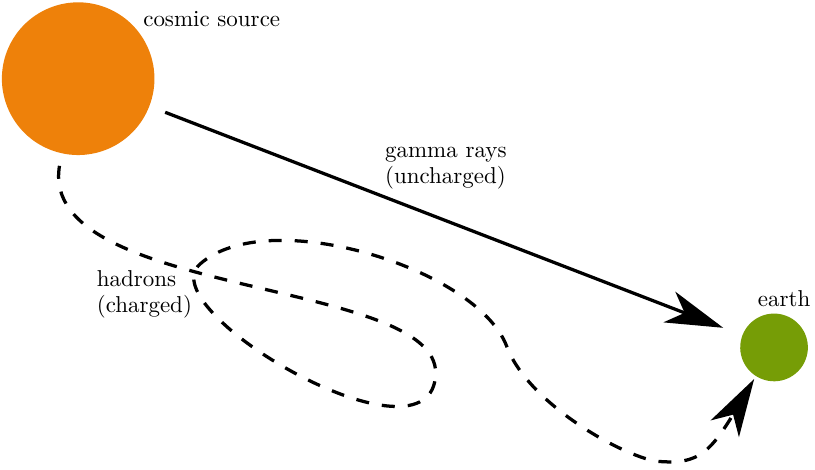
\includegraphics[width=10cm, keepaspectratio]{Screenshot_20171128_100930.png}
\caption{}
\label{fig:cosmic}
\end{subfigure}
\hfill
\centering
\begin{subfigure}[t]{1\textwidth}
  \centering
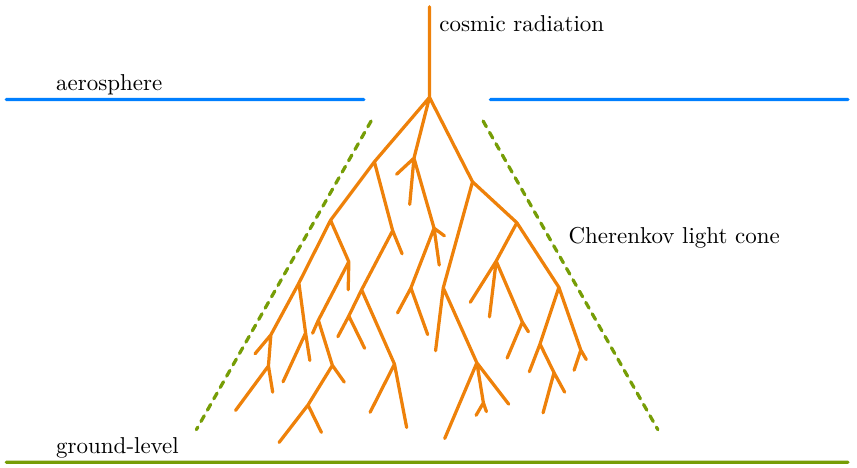
\includegraphics[width=10cm, keepaspectratio]{Screenshot_20171128_101617.png}
\caption{}
\label{fig:airshower}
\end{subfigure}
\caption{(a) Gamma-rays and Hadrons as they propagate through space. (b) Illustration of an air shower\cite{behnken_2017}.}
\end{figure}

Gamma-rays and hadrons are detected through a process called Cherenkov radiation. Cherenkov radiation is light that is emitted by particles that are moving incredibly fast in a medium, such as the air or water. For Cherenkov radiation to happen, the particles have to be moving faster than the local speed of light, which is the speed of light divided by the index of refraction for that medium. As long as the particle moves faster than the local speed of light, Cherenkov radiation will be emitted in the direction the particle is moving, creating a narrow cone of light.

For gamma-rays and hadrons, when they enter the atmosphere they not only are moving faster than the local speed of light, but also interact with air molecules. Those interactions produce more particles that produce more light cones. The end result is a shower of Cherenkov radiation that can be detected by instruments such as FACT. An illustration of the process is shown in Fig. \ref{fig:airshower}. The gamma-ray and proton events usually create slightly different showers in the detector, enabling the ability to discriminate between the two event types. 



\subsection{First G-APD Cherenkov Telescope (FACT)}\label{sec:FACT}

The FACT telescope is the first operational telescope of its kind, using a camera equipped with a hexagonal grid of silicon photo multipliers (G-APD aka SiPM) to primarily detect gamma rays\cite{ANDERHUB2011107}. Photo multipliers work by absorbing photons and emitting electrons that generate a current that can be read out by the hardware to determine how many photons have hit the photo multiplier. Located in La Palma in the Canary Islands, FACT has been operational since 2011 and during that time has done near-continuous observations of the night sky. The FACT telescope works by using the SiPM's to detect showers of photons created when gamma-rays or hadrons impact particles in the atmosphere. The details of such showers are explained in \ref{sec:gammaVhadron}.

\subsubsection{Imaging Air Cherenkov Telescope (IACT)}\label{sec:cta}

An Imaging Air Cherenkov Telescope is a type of telescope that is designed to detect very high energy gamma ray photons through detecting showers of Cherenkov radiation. There are a few currently working IACTs, including HESS\cite{2004NewAR..48..331H} in Nambia, MAGIC\cite{aleksic2016major} located in La Palma in the Canary Islands, VERITAS\cite{park2015performance} in Arizona, and FACT\cite{1748-0221-8-06-P06008} located next to MAGIC in La Palma. HESS, MAGIC, and VERITAS are all comprised of arrays of IACTs, while FACT is composed of a single telescope. FACT's original status as a technology demonstrator for SiPMs lead it to be constructed as a single telescope, while most other IACTs are arrays of telescopes to eliminate background events.

One of the largest next generation gamma-ray telescope projects is the Cherenkov Telescope Array, or CTA, that is comprised of multiple IACT of various sizes built into an array for better sensitivity. With an expected online date of 2024, CTA is still years away from operation, but lessons learned with improving FACT's event classification could improve CTA's classification.

\subsection{Neural Networks}\label{sec:NN}

Neural networks are a type of computer program that can be used to classify inputs into various categories depending on their structure. There are various ways to create neural networks. In this thesis, convolutional neural networks (CNN) will be investigated to see how effective they are at classifying FACT data compared to the current Random Forest approach.

\subsubsection{Convolutional Neural Network}\label{sec:cnn}

Convolutional Neural Networks are one of the most common types of neural networks used. This type of network tends to do very well at image tasks. 

CNNs are composed of multiple layers that do different tasks. Convolution layers act to find patterns and features in the input image. Pooling layers take the output from other layers, such as convolutional ones, and act to select the most important features from the previous layers. Finally, fully connected layers take the output from the previous layers and combine the features and patterns found to classify the image, in this case as either a gamma-ray event or a hadron event. There are also other types of layers, such as dropout layers that stops some of the information from previous layers from continuing through the network, so that the network does not overfit to the training data. CNNs can be comprised of multiple convolutional, pooling, fully connected, and dropout layers in different orders to classify inputs in different ways. 

The deep learning library used for this thesis will be Google's TensorFlow\cite{tensorflow2015-whitepaper}. It can be set up in various ways and integrates with Python. All the neural networks will be written using this library or potentially in a library called Keras\cite{chollet2015keras}, which simplifies some of the steps needed to get a network up and running, but still uses Tensorflow for the backend.

\subsection{Monte Carlo Simulation}\label{sec:mc}

Monte Carlo simulations are a very important part of training current classifiers and understanding gamma-ray and hadron air showers. The simulations try to accurately recreate different initial conditions that result in either a gamma-ray event or a hadron event. The simulations contain detailed information about every aspect of the event that it simulates, such as the photon energy, initial starting point, the effects of the detector, and as much other information as possible. One issue with the Monte Carlo simulations is that the simulations do not perfectly replicate the physics of the different events. As of this writing, the Monte Carlo events that the FACT collaboration uses differ slightly in some parts of the event shapes, frequency of events, and timing information, among other mismatches. Because of these discrepancies between the physical system and the Monte Carlo simulations, there is the problem of Monte Carlo Mismatch, where the classifier learns to differentiate the two event types using information that is not contained in the real data, but only the Monte Carlo resulting in poor classification. 

\subsection{Current Approach}\label{sec:current}

The current approach to classifying the gamma/hadron events for FACT uses a Random Forest classifier\cite{fact_classifier}. A Random Forest is an ensemble of decision trees that classifies input based on the combined output from multiple different decision trees. A Decision Tree is a way to classify input based on multiple parameters. It is essentially like a flow chart, comprised of true/false decisions ultimately resulting in a final classification and confidence level. The benefits of a decision tree is that it is a white box, as in the entirety of how it works is right out in the open. The current classifier uses an ensemble of 200 trees that classify the input based on the shape, number of photons, timing information, and other spatial and temporal information.

\section{Proposal}\label{sec:proposal}

The hypothesis of this study is that an improvement over the current classifier for FACT can be implemented using a neural network.

\subsection{Previous Work}\label{sec:previous}

The starting point for this thesis is the Bachelor's thesis of Jan Morwitz \cite{behnken_2017}, who also tried to improve the classification using a CNN. His results were somewhat disappointing in that the CNNs performed slightly worse than the current classifier. His approach also left multiple ways for improvement, which this thesis explores to some extent as part of its methods. One of the main issues presented in his thesis is the mismatch between the simulation data and the real data, a key point this thesis explores and is described in \ref{sec:mc}.

There has been other work in using Neural Networks to classify gamma/hadron events. The MAGIC, VERITAS, and HESS telescopes have also been working on integrating neural networks into their gamma/hadron classification\cite{2006APh....25..380K, boinee2006neural, murach2015neural}, although their approaches are different from what is done in this thesis as they incorporate information from multiple different telescopes in an array, instead of the single FACT.

There has also been work in discriminating between hadron and gamma-ray events through the spatial development of the air showers combined with their temporal development. When combined with other discriminators, such as the $\theta^2$ cut\footnote{The square of the angular difference between the reconstructed air shower position and the source position.} there was an improvement over approaches that don't include timing information\cite{prokoph2009investigations}. These approaches show that as more information is included in approaches to separate the event types, it tends to result in better event classification.

For the Cherenkov Telescope Array, described in \ref{sec:cta}, there has been research into classifying events even though the array will not be active until the mid 2020s. With CTA's multiple telescopes, it can record both two-dimensional air shower images from a single telescope in the array, or three-dimensional images of an air shower by combining multiple images from individual telescopes in the array. Using Monte Carlo simulation data, there has been recent work on using both these two-dimensional and three-dimensional air shower images and convolutional neural networks to attempt to improve classification over current methods\cite{2017arXiv170905889N}. One group also split up the data into different energy bands and trained networks on those. This preliminary CTA work, though, has been somewhat inconclusive, with networks overfitting to the data and the different energy bands resulting in significantly different results\cite{2017arXiv171106298L}. In addition, because CTA currently has no real data to compare to, the results from its classification should be taken with a grain of salt, as the Monte Carlo simulations might not be physically accurate.

\subsubsection{Non Neural Network Approaches}

While Neural Networks are the focus of this thesis, and of intense interest to the computer science and physics communities at large, there are other types of machine learning techniques that have been or are currently used for gamma/hadron separation. The most common is the Decision Tree approach, whereby features of the gamma ray and hadron showers are chosen and built into trees that classify events as one type or another based on the existence or absence of the features in the data. This is the approach taken by the current FACT analysis pipeline and described in \ref{sec:current}.

Another approach is a technique called support vector machines. In this approach, the algorithm maps input data to high-dimensional space, and finds a plane that separates that space between points known to be hadron-generated events and gamma-ray-generated events. For example, while in two-dimensional space two sets of points may overlap, in three-dimensional space they might be easily separable, as in Fig. \ref{fig:svm}. For gamma/hadron separation, though, support vector machines have tended to do worse than random forests\cite{boinee2005ensembling}.

\begin{figure}[!htb]
\centering
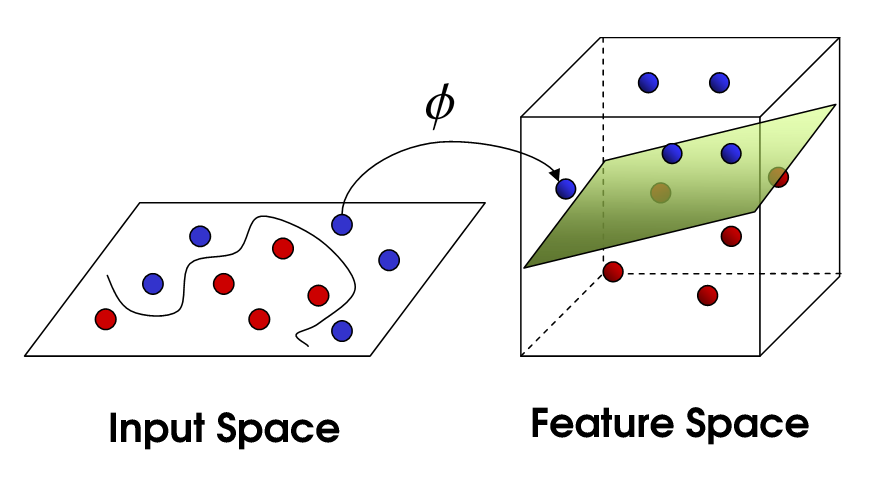
\includegraphics[width=8cm, keepaspectratio]{svm.png}
\caption{Support Vector Machine Visualization.}
\label{fig:svm}
\end{figure}

\section{Method}\label{sec:method}

The first part of this thesis will investigate how training the random forest classifier on real data affects its results. The new training will use Crab Nebula observations as the ground truth gamma-ray events and background observations for the hadron events. If the new training regime results in a classifier that works as well as the classifier trained on Monte Carlo events, then any discrepancies between the two classifications will be examined. For events that each classifier classifies with a confidence of 0.9 or better, discrepancies will be examined to see what the differences are between them. In addition, events that both classifiers classify at 0.9 confidence or better will be used for training neural networks, replacing Monte Carlo events for training. Both classifiers will be tested on a real dataset and a Monte Carlo dataset to determine their accuracy. 

After comparing the current classifier trained on real data and Monte Carlo data, real events that both classifiers rate as either a gamma-ray or hadron event with 90\% confidence or better will be used as training data for different neural networks. Convolutional Neural Networks are the only type of network that will be tested in this thesis. The previous work's CNN will be trained with the new training data and compared to other networks that take advantage of more temporal or spatial information, such as the timing of photons arriving at the detector or a better spatial representation of the hexagonal grid. As the networks expand in dimensionality, more information can be included in the classification at the risk of overfitting the model to the training data and at larger and larger computational cost. 

After the networks are trained, they will be tested on both real and simulated events and compared to the current classifier and the one trained in the first step of the thesis. 

\subsection{Proposed Improvements}

There are various improvements that can be applied to see what improves the classification.

\subsubsection{Changing Training Data}

The first improvement to try is to change the training data from Monte Carlo data to solely real data.

For neural networks, the data that is used to train the network significantly affects how accurate it is when used to classify events. Up until now, the CNNs used for the FACT data have been trained entirely on Monte Carlo simulation data, or a mixture of Monte Carlo data and real hadron events. Some IACTs such as the MAGIC telescopes use such a mixture of real and simulated data when training their classifier\cite{albert2008implementation}. While the simulation data is designed to be physically accurate and the same as the real observation data, there are discrepancies and extra information that are not contained in the real data, but is in the Monte Carlo data. These differences can lead to misclassifications and poorer performance.

One way to eliminate errors in the classification from the Monte Carlo data is to switch to using all real data to train the network. The downsides of using real data versus Monte Carlo is that real data has uncertainties and there is not a guarantee that a gamma event or a hadron event in the real data is actually that event type. In Monte Carlo, we have all the information about every particle contained in the simulation, so there is no uncertainty about an event type. To try to overcome this limitation, this thesis will use only real data that is classified as having at least a 90\% confidence of being one event type or another by both the Random Forest classifier trained on the Monte Carlo data and the classifier trained on real data. 

\subsubsection{Changing Mapping}

Another improvement would be to change how the hexagonal FACT sensor is mapped into a format that TensorFlow can use. Most programming languages have problems with input that is hexagonal, as most are built to handle regular grid patterns, such as the array of pixels that make up a computer screen or digital camera sensor. Since FACT uses a hexagonal grid, there are a few ways that such a grid can be transformed into something that TensorFlow and other programs can easily use. The previous work mapped the hexagons to a regular grid, as shown in Fig.\ref{fig:gridCompare}. In that process, though, some information was lost. In a hexagonal grid, each point has six neighbors, but in a regular grid, the number of neighbors decreases to four, removing a third of the neighbor information for each pixel from the final image. In contrast, if a hexagon is converted into a three-dimensional cube, then it still has six neighbors and no neighbor information is lost. In addition, a hexagon is a slice from a cube, so converting each hexagon to a cube results in no loss of information. Since having more information for the network to train on is generally better, keeping more of the original information should lead to better classification.

\begin{figure}[!htb]
\centering
\begin{subfigure}[t]{.475\textwidth}
  \centering
  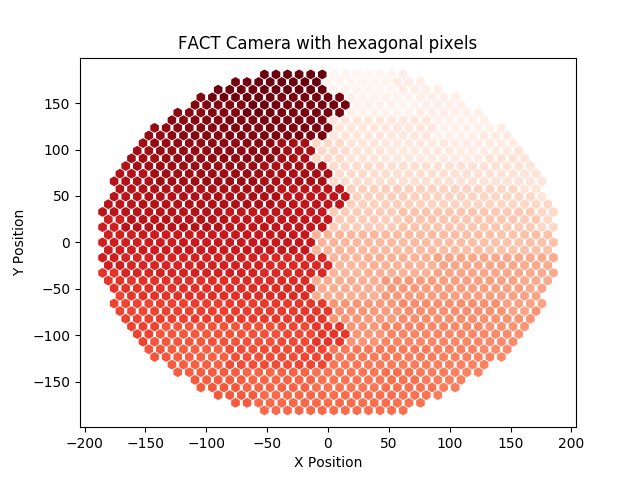
\includegraphics[width=8cm, height=8cm, keepaspectratio]{Unskewed_Mapping.png}
  \caption{Original camera pixel grid.}
  \label{fig:Unskewed}
\end{subfigure}
\hfill
\begin{subfigure}[t]{.475\textwidth}
  \centering
  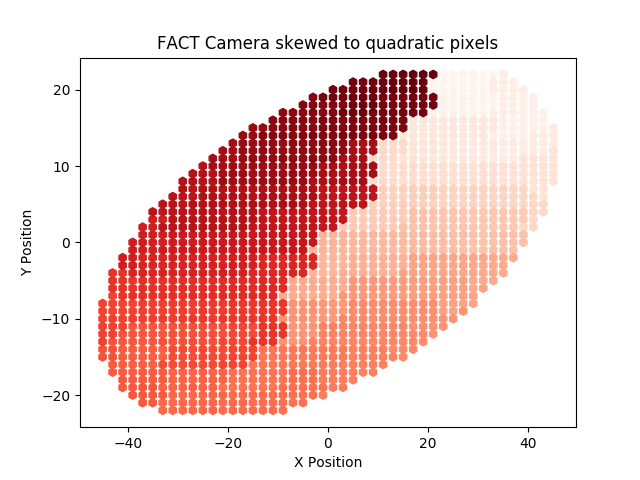
\includegraphics[width=8cm, height=8cm, keepaspectratio]{Skewed_Mapping.png}
  \caption{Skewed camera grid.}
  \label{fig:Skewed}
\end{subfigure}
\centering
\begin{subfigure}[t]{.475\textwidth}
  \centering
  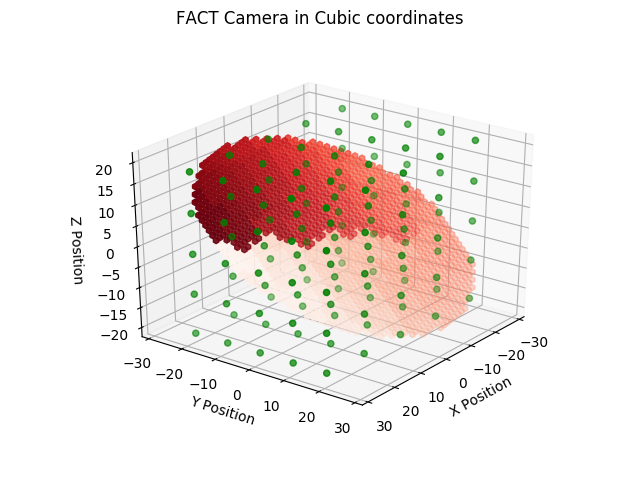
\includegraphics[width=8cm, height=8cm, keepaspectratio]{Cubic_Mapping_FACT_Face.png}
  \caption{Camera grid mapped to 3D cubic pixels, face on. Green points are to show the cube that the hexagons are cut from.}
  \label{fig:CubeEdge}
\end{subfigure}
\hfill
\begin{subfigure}[t]{.475\textwidth}
  \centering
  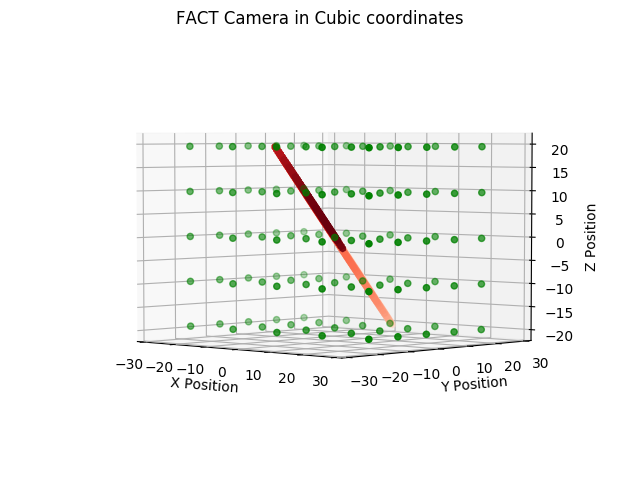
\includegraphics[width=8cm, height=8cm, keepaspectratio]{Cubic_Mapping_FACT_Edge.png}
  \caption{Camera grid mapped to 3D cubic pixels, edge on, showing how a hexagonal grid is a slice through 3D cube space.}
  \label{fig:CubeFace}
\end{subfigure}
\caption{Example of changing the mapping of pixel from hexagonal to quadratic and cubic coordinate systems. Color indicates the hardware ID of each of the 1440 pixels.}
\label{fig:gridCompare}
\end{figure}

\subsubsection{Higher Dimensional Convolutions}

In a similar way to changing the mapping from two dimensional to three dimensional should improve the classification because of more information, going from two dimensional convolutions to three dimensional ones should have a similar effect. The two three dimensional convolutions that are currently planned would be doing a convolution over space -- the cube that the hexagon maps to -- and then a convolution over time, using the two dimensional mapping, but instead of summing the photons, leaving the input as a stack of images. 

The convolution over time and space partly depends on the two convolutions actually improve the classification or not. If one or both do, then combining them, so that the convolutions go over both time and space should give the best results, as all available information is then used by the neural network to classify images.

\section{Timeline}\label{sec:timeline}

The timeline for the thesis is roughly as shown below. As of this prospectus, the previous work has been replicated, the decision tree is being trained on the real dataset, and initial work on a 3D CNN has been started. 

\begin{table}[!htb]
\renewcommand\arraystretch{1.4}\arrayrulecolor{LightSteelBlue3}
\captionsetup{singlelinecheck=false, font=blue, labelfont=sc, labelsep=quad}
\caption{Timeline}\vskip -1.5ex
\begin{tabular}{@{\,}r <{\hskip 2pt} !{\foo} >{\raggedright\arraybackslash}p{5cm}}
\toprule
\addlinespace[1.5ex]
Summer 2017 & RISE Internship, develop idea and get access to dataset\\
Dec 2017 & Recreate previous work, train new Random Forest classifier\\
Jan 2018 & Have tested Random Forest classifier, selected new training data, build CNNs\\
Feb 2018 & Train neural networks, try different improvements to the networks\\
March 2018 & Compare CNNs and default results\\
April 2018 & Finish up results, finish thesis\\
May 2018 & Thesis Defense\\
\end{tabular}
\end{table}

\newpage
\newpage
\nocite{*}
\printbibliography

\end{document}
